\section{Introduction}
\label{sec:intrp}

%Purpose
%- what is the micro:bit?
% http://www.bbc.co.uk/programmes/articles/4hVG2Br1W1LKCmw8nSm9WnQ/the-bbc-micro-bit

The micro:bit is a small programmable and embeddable computer designed, 
developed and deployed by the BBC and partners (including ARM, Microsoft
and Lancaster University) to approximately 800,000 UK middle school students
in 2015-2016. Part of the BBC's Make It Digital Campaign, the BBC described the
micro:bit as its ``most ambitious education initiative in 30 years, 
with an ambition to inspire digital creativity and 
develop a new generation of tech pioneers.''~\cite{BBCwebsite}

% reference the competition and show what's different (hardware)
% https://barrettsprojects.wordpress.com/2012/09/15/tap-and-double-tap/ 

Figure~\ref{fig:microbit} shows (a) the front and (b) the back of the
micro:bit, which measures 4cm x 5cm. Like the Arduino Uno, 
the micro:bit is a single-board microcontroller 
that can be programmed via a host computer (usually a laptop or desktop)
and then embedded in projects where it runs on battery power.
In contrast to the Uno, which has no built-in sensors, the micro:bit 
board hosts a variety of sensors (temperature, accelerometer, magnetometer, 
light level), 
a 5x5 LED matrix, two user-defined buttons, as well as Bluetooth
Low Energy (BLE) communications.\footnote{The micro:bit has a whopping
16kB of RAM and 256kB of Flash memory, compared to the Uno's 2kB of 
RAM and 32kB of Flash}.

The design of the micro:bit hardware was driven by the
first two objectives of the BBC micro:bit project:
(B1) to provide a simple creative experience for physical computing, wearable and Internet of Things (IoT) projects;
(B2) to supply a device that can continue to provide learning opportunities as the user's expertise grows.

On the hardware side, the micro:bit's built-in sensors, buttons and LED display 
allow many projects to be completed with no additional hardware or wiring. 
The holes on micro:bit's edge
connector allows additional external sensors and actuators to be connected via crocodile clips.
The micro:bit's BLE capabilities introduces networking to the
picture, and enables streaming of data and command/control operations among the micro:bit, 
smartphones, laptops, as well as other micro:bits.
As with Arduino, an ecosytem of micro:bit shields
(hardware peripherals) that accommodate the micro:bit's edge
connector expands its capabilities greatly.\footnote{
\url{http://microbit.org/assets/documents/AccessoryGuideSummer18.pdf}
}

\begin{figure} 
\begin{tabular}{cc}
  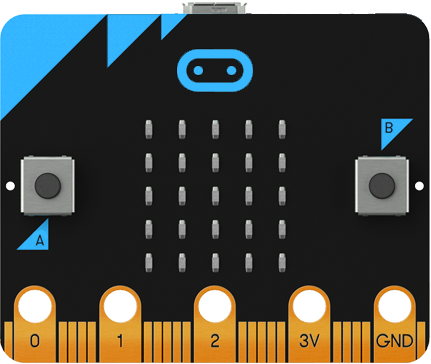
\includegraphics[width=1.5in]{images/microbit-front.png} &
  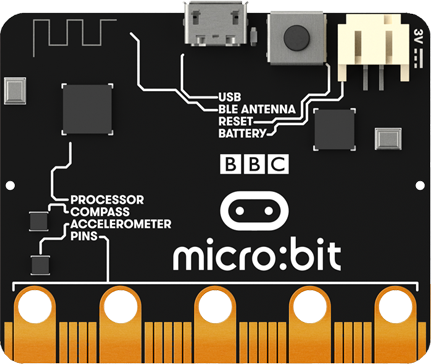
\includegraphics[width=1.5in]{images/microbit-back.png} \\
  (a) & (b) 
\end{tabular}
\caption{\label{fig:microbit}The micro:bit: (a) front, with two buttons, 
  5x5 LED display, and edge connector (bottom); (b) back, with processor, accelerometer, compass, Bluetooth, USB and battery ports.}
\end{figure}

% micro:bit is an embeddable, reactive, networked computing system

The design of the micro:bit coding tools also was oriented towards a 
simple starting experience with room for progression. In particular, the coding 
objectives of the project were: (B3)
to give students an exciting, engaging introduction to coding;
(B4) to stimulate curiosity about how computing technologies can be utilized 
  to solve problems that students identify. 

  \begin{figure*}[t] 
    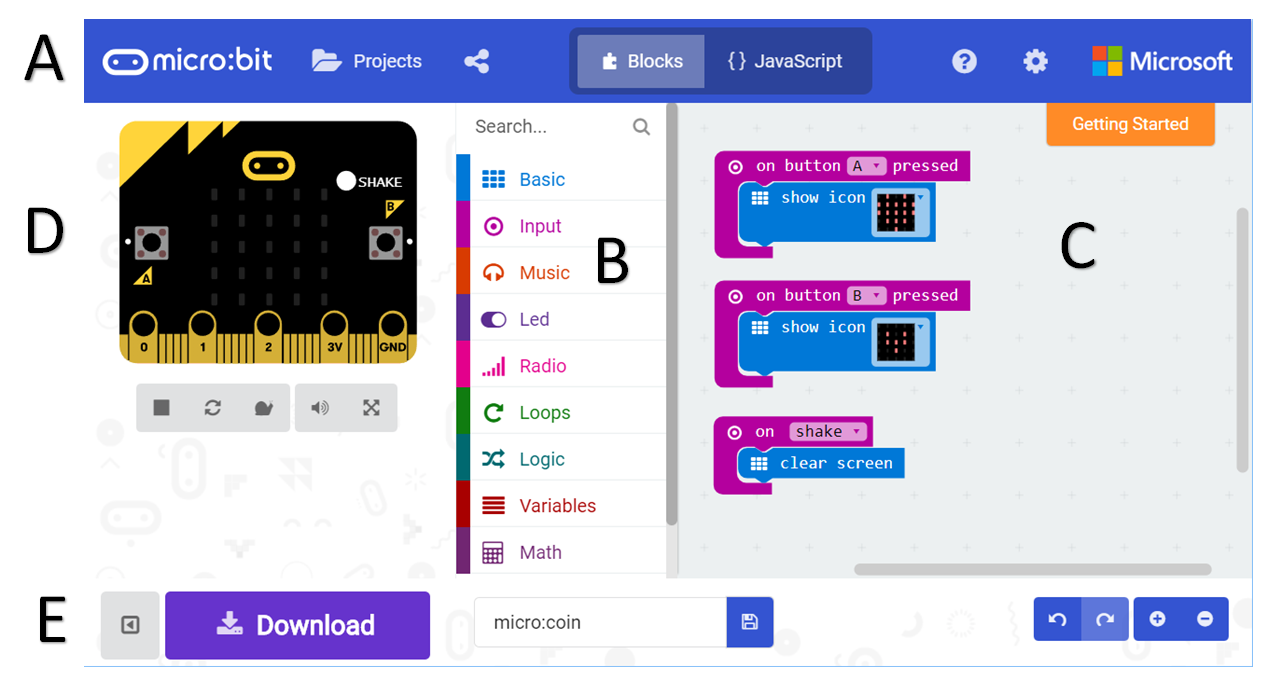
\includegraphics[width=6in]{images/webApp.png}
    \caption{\label{fig:snapshot}MakeCode web app for the micro:bit}
\end{figure*}

Based on user trials with a micro:bit prototype with students in Years 5 and 7 (3rd and 5th grade
in the US, respectively), the BBC focused on delivering a web app 
based on the popular Blockly framework~\cite{Blocky2015} to permit students to
create scripts via drag-and-drop operations in a web browser, and see
the execution of their scripts via a simulator.
Text-based coding via scripting languages also 
was identified as an important feature. As the micro:bit would be incorporated 
into standalone projects, it also was essential for the user's program to be 
compiled and installed in non-volatile storage on the micro:bit where it 
could be run via battery power.

%final design put the entire toolchain in web app, without need to invoke C/C++ compiler to
%compile the user's program; ARM DAPlink solution makes micro:bit appear as USB pen drive
%on all operating systems; MicroPython provided second programming solution with entire toolchain
%on the micro:bit!!]

The solution delivered by the BBC's partners evolved from the initial
design to include:
\begin{itemize}
\item support for Blockly, JavaScript, Python and C++;
\item an efficient C++ runtime for the micro:bit created by Lancaster
University;
\item a web app (\url{http://makecode.microbit.org})
with Blockly and JavaScript editors, micro:bit simulator, 
and a compiler to machine code, linked against a pre-compiled C++ runtime;
\item a Python compiler and read-eval-print loop (REPL) that resides
{\em on the micro:bit} (via \url{https://micropython.org/}), 
supported by a simple web app (\url{http://python.microbit.org}) and 
an installable application (\url{https://codewith.mu/});
\item ARM's DAPlink firmware makes the micro:bit appear as USB pen drive 
on most operating systems, enabling a simple file copy operation to 
install a user's program on the micro:bit (no device drivers needed).
\end{itemize}
MakeCode, MicroPython, and the C++ runtime are all open source.\footnote{
At \url{https://github.com/microsoft/pxt},
\url{https://github.com/micropython/micropython},
and \url{https://github.com/lancaster-university/microbit-dal}, 
respectively.}

Figure~\ref{fig:snapshot} shows a screen snapshot of the MakeCode web app
for the micro:bit with five main sections: (A) menu bar with access to projects
and examples, and switching between Blockly and JavaScript editors; (B)
Blockly toolbox of micro:bit API categories; (C) Blockly programminng
canvas with a simple reactive program; (D) micro:bit simulator for execution
of the user's program in browser; (E) download button, which invokes the in-browser
compiler to produce a binary executable. 

The event-based program shown in section (C) displays a large heart when the
A button is pressed, displays a small heart when button B is pressed,
and clears the display when the user shakes the micro:bit (shake
detection is implemented using the accelerometer; in the simulator, the
shake event is fired using a virtual button). In addition to event-based
APIs, direct access to the micro:bit's sensors via polling is possible.
[takes a few minutes to code and deploy this simple program]

The BBC micro:bit project also called for partners to develop content
and to ``train the trainers'' (educators) around the micro:bit computing
system.

%- A lot of lessons learned from delivering end-to-end experience in UK and other countries
%   - hardware (unique design, as already mentioned)
%   - firmware:  high-level C/C++ runtime and ARM's DAPlink
%   - web-based IDE: no C/C++ compiler needed to compile user code
%   - content
%   - training
% In country partnerships

In the remainder of this paper, we focus on the primary promise
of the BBC micro:bit, which was to deliver a simple physical computing
experience for beginners and a progression path for users to follow
as their expectations increase. [micro:bit education foundation founded
in the fall of 2016]  We draw from two full years of 
full deployment of the micro:bit in the UK, as well as deployments
in Europe, the United States, and Asia.  There are approximately
two million micro:bits now in the market and many hardware,
content, and education partners participating. 



Overview: Section~\ref{sec:physical} on physical computing;


% compared to Arduino
% https://twitter.com/adamwwolf/status/1019070808038072320



% success of micro:bit due to 
% - Low-cost, simplicity
% - Partnerships (hardware, software, content, training)
% - Open Source of software (CODAL, MakeCode, ...)
% - Hardware Reference design

% - why is it interesting?
%   - edge/physical/IoT computing
%   - build off of Scratch/Blockly, but untethered (via in-browser compiler)
%   - transition to JavaScript and Python

% - BBC rollout in UK
% - Global reach
%    - BBC rollout mirrored in other countries
%    - Communities
%      - Sri Lanka user group: http://microbitslug.org/
%      - UK libraries (loan program)
%    - third party editors









